\documentclass[conference]{IEEEtran}
\IEEEoverridecommandlockouts

\usepackage{iftex}
\ifXeTeX % local XeTeX builds: use a Times clone so the layout matches pdfLaTeX on Overleaf
  \usepackage{fontspec}
  \setmainfont{texgyretermes}[Extension=.otf, UprightFont=*-regular, BoldFont=*-bold,
    ItalicFont=*-italic, BoldItalicFont=*-bolditalic]
\fi
\usepackage{cite}
\usepackage{amsmath,amssymb,amsfonts}
\usepackage{graphicx}
\usepackage{booktabs}
\usepackage{multirow}
\usepackage{array}
\usepackage{xcolor}
\usepackage{url}
\usepackage{tikz}
\usetikzlibrary{positioning,arrows.meta,fit,calc,backgrounds}

\graphicspath{{figures/}}

% Diagram styles
\tikzset{
  blk/.style={draw, rounded corners=2pt, align=center, font=\scriptsize, minimum height=8.5mm, inner sep=2pt, fill=white},
  sDATA/.style={blk, fill=blue!7},
  sPROC/.style={blk, fill=orange!10},
  sNET/.style={blk, fill=green!9},
  sOUT/.style={blk, fill=red!8},
  arr/.style={-{Stealth[length=1.6mm]}, semithick},
  lane/.style={draw=gray!60, dashed, rounded corners=3pt, inner sep=4pt},
  lanelabel/.style={font=\scriptsize\itshape, text=gray!70!black, anchor=south west},
}

\newcommand{\cmark}{\checkmark}
\newcommand{\xmark}{$\times$}

\begin{document}

\title{A Standards-Compliant, Inter-Patient Evaluated Lightweight ECG Arrhythmia Classifier for Resource-Constrained Embedded Deployment}

\author{
\IEEEauthorblockN{Nabarun Dey}
\IEEEauthorblockA{School of Computer Engineering\\
Manipal Institute of Technology\\
MAHE, Manipal, India\\
Reg. No. 240911236\\
{\footnotesize nabarun.mitmpl2024@learner.manipal.edu}}
\and
\IEEEauthorblockN{Jerome Varghese}
\IEEEauthorblockA{School of Computer Engineering\\
Manipal Institute of Technology\\
MAHE, Manipal, India\\
Reg. No. 240911430\\
{\footnotesize jerome.mitmpl2024@learner.manipal.edu}}
\and
\IEEEauthorblockN{S. Durgaprasad}
\IEEEauthorblockA{School of Computer Engineering\\
Manipal Institute of Technology\\
MAHE, Manipal, India\\
Reg. No. 240911023\\
{\footnotesize durgaprasad.mitmpl2024@learner.manipal.edu}}
}

\maketitle

\begin{abstract}
Deep-learning ECG arrhythmia classifiers routinely report accuracies above 95\%, yet only 5 of 122 recent studies simultaneously follow the AAMI EC57 standard, evaluate on patients unseen during training, and assess embedded feasibility. We design, train and evaluate a lightweight one-dimensional convolutional neural network (1D-CNN) that meets all three criteria. Each heartbeat of the MIT-BIH Arrhythmia Database is classified into the five AAMI classes from its single-lead morphology and eight RR-interval features expressed relative to the patient's own rhythm. Training uses only the DS1 records; every design choice is made on a patient-wise validation hold-out from DS1, and the DS2 records serve as the inter-patient test set. The final model is an ensemble of three 4,974-parameter networks, each quantized to 8-bit integers. On DS2 it reaches 87.30\% accuracy, an SVEB sensitivity of 74.46\% with 33.43\% positive predictivity, and a VEB sensitivity of 92.89\% with 92.71\% positive predictivity. The ensemble needs 15.1~KB of INT8 weights, 0.76~million multiply-accumulates per beat and about 3.9~KB of peak activation memory, under 1\% of the 520~KB SRAM of an ESP32-WROOM-32E. INT8 quantization costs 0.1 percentage points of accuracy against the float ensemble. Error analysis attributes 86.5\% of SVEB false alarms to five test patients with atrial fibrillation or 2:1 AV block. An ablation shows that a rhythm-irregularity feature raises SVEB positive predictivity to 42.31\%. This gain could not be detected by our validation set, which contains no atrial-fibrillation records.
\end{abstract}

\begin{IEEEkeywords}
ECG, arrhythmia classification, AAMI EC57, inter-patient evaluation, 1D-CNN, quantization, embedded systems, TinyML
\end{IEEEkeywords}

%=====================================================================
\section{Introduction}
%=====================================================================
Cardiovascular diseases are the leading cause of death worldwide, accounting for an estimated 19.8~million deaths in 2022~\cite{who2025cvd}. Arrhythmias, abnormal or irregular heartbeats, are a key indicator of cardiac health, and their early detection can substantially improve outcomes. The electrocardiogram (ECG) is the standard non-invasive tool for this, but beat-by-beat inspection of long recordings is slow and error-prone. Wearable patches, Holter monitors and implantable loop recorders make continuous monitoring outside hospitals practical, which creates demand for classifiers that run directly on small, low-power devices~\cite{silva2026review,demeloribeiro2022quantized,busia2025tiny}.

Many deep-learning studies report accuracies above 95\%~\cite{xiao2023review}, but these figures are often not comparable and do not transfer to deployment, for two reasons. First, the AAMI EC57 standard~\cite{aami2012ec57} defines the beat classes and metrics but not how data are partitioned. Many studies mix beats of the same patient in training and test sets (the \emph{intra-patient} paradigm), so a model can memorize patient-specific morphology. In the \emph{inter-patient} paradigm of de Chazal et al.~\cite{dechazal2004automatic}, training and test patients are disjoint, and performance drops sharply, especially for clinically important minority classes. Second, many accurate models are too large for microcontroller memory, energy and latency budgets, and most papers never measure this. Silva et al.~\cite{silva2026review} combine these concerns as the E3C criteria (Embedded, Clinical and Comparative). Of 122 studies, only 5 (4.1\%) satisfy all three (Fig.~\ref{fig:e3c}).

\begin{figure}[t]
\centering
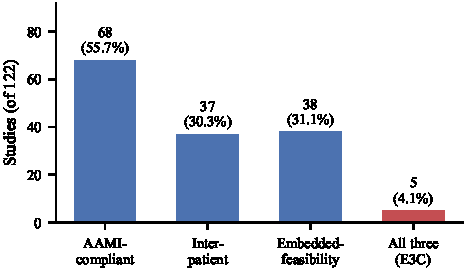
\includegraphics[width=\columnwidth]{e3c_adherence}
\caption{Adherence of the 122 studies reviewed in~\cite{silva2026review} to the three deployment-relevant criteria.}
\label{fig:e3c}
\end{figure}

This work addresses that gap. Our contributions are:
\begin{itemize}
\item an AAMI-compliant 1D-CNN with patient-relative RR features, trained on DS1 and tested on the canonical DS2 split, with every model choice made on a patient-wise validation hold-out;
\item full INT8 post-training and quantization-aware compression, with model size, operation count and peak activation memory measured against an ESP32-WROOM-32E budget;
\item a three-member INT8 ensemble that removes the large seed-to-seed variance of minority-class results at a cost of 15.1~KB of weights;
\item an error analysis tracing SVEB false alarms to atrial fibrillation (AF), with ablations of a rhythm-irregularity feature and of a causal (zero-latency) variant; and
\item a transparent account of every use of the test set during development, together with a frozen, checksummed final model.
\end{itemize}

%=====================================================================
\section{Related Work}
%=====================================================================
\subsection{Standards and Evaluation Protocol}
ANSI/AAMI EC57~\cite{aami2012ec57} groups MIT-BIH beat types into five superclasses: normal (N), supraventricular ectopic (SVEB), ventricular ectopic (VEB), fusion (F) and unknown (Q). It recommends excluding paced recordings and reporting sensitivity (Se), positive predictivity (+P) and false positive rate (FPR) alongside accuracy. MIT-BIH~\cite{moody2001impact,goldberger2000physiobank} holds 48 half-hour two-lead recordings at 360~Hz from 47 patients. Surveys~\cite{xiao2023review,luz2016survey} agree that intra- and inter-patient results are not comparable and that the inter-patient paradigm is the reference for claims about unseen patients. Because about 89\% of beats are normal, accuracy is dominated by class N; per-class Se and +P are the informative metrics.

\subsection{Accuracy-Oriented and Lightweight Models}
Kiranyaz et al.~\cite{kiranyaz2016realtime} showed that compact 1D-CNNs can classify beats in real time. Large models such as the deep residual network of Ribeiro et al.~\cite{ribeiro2020automatic} or the transformer of Hu et al.~\cite{hu2022transformer} (about 20~MB~\cite{busia2025tiny}) show what unconstrained models achieve but are not microcontroller-class. Among edge-oriented work, DL-LAC~\cite{sakib2021ultraedge} measured time and memory on virtualized microcontrollers. Seitanidis et al.~\cite{seitanidis2022edge} deployed a 2D-CNN on a Jetson Nano but used a random 80/20 split. De Melo Ribeiro et al.~\cite{demeloribeiro2022quantized} quantized a 1D-CNN to 93~kB under an intra-patient protocol. Busia et al.~\cite{busia2025tiny} ran a 6,649-parameter INT8 transformer on GAP9 in 4.28~ms and 0.09~mJ, again with a shuffled beat-level split. Kim et al.~\cite{kim2024ultraedge} met all three E3C criteria with a 25~kB model using 118~kB RAM on a Cortex-M4, but with a custom subject partition. Farag~\cite{farag2023tiny} reported an inter-patient, 15~kB quantized CNN, but on a Raspberry Pi with 12--24~MB runtime memory. Saha Tchinda and Tchiotsop~\cite{sahatchinda2025lightweight} evaluated a light 1D-CNN inter-patient but gave no embedded analysis. Table~\ref{tab:e3c} summarizes these studies.

\subsection{Compression}
Integer-only quantization~\cite{jacob2018quantization} maps weights and activations from 32-bit floats to 8-bit integers and is the most common choice for microcontrollers~\cite{demeloribeiro2022quantized,busia2025tiny}. Lin et al.~\cite{lin2022ondevice} illustrate how tight practical memory limits are (256~kB). The ESP32-WROOM-32E offers 520~kB of on-chip SRAM and 4--16~MB of flash~\cite{espressif2023esp32}.

\begin{table}[t]
\caption{Selected Studies Versus the Three E3C Criteria}
\label{tab:e3c}
\centering
\footnotesize
\setlength{\tabcolsep}{3pt}
\resizebox{\ifdim\width>\columnwidth\columnwidth\else\width\fi}{!}{%
\begin{tabular}{@{}llccl@{}}
\toprule
Ref. & Model & AAMI & Inter-pat. & Embedded evidence \\
\midrule
\cite{sahatchinda2025lightweight} & 1D-CNN (light) & \cmark & \cmark & None reported \\
\cite{demeloribeiro2022quantized} & 1D-CNN, INT8 & \cmark & \xmark & 93~kB model \\
\cite{seitanidis2022edge} & 2D-CNN & \cmark & \xmark & Jetson Nano \\
\cite{busia2025tiny} & Tiny transformer & \cmark & \xmark & GAP9, 0.09~mJ \\
\cite{sakib2021ultraedge} & 1D-CNN (DL-LAC) & \cmark & \xmark & Virtual MCU \\
\cite{kim2024ultraedge} & 1D-CNN, INT8 & \cmark & \cmark$^{a}$ & Cortex-M4, 118~kB RAM \\
\cite{farag2023tiny} & Matched-filter CNN & \cmark & \cmark & 15~kB, Raspberry Pi \\
\midrule
This work & 1D-CNN ens., INT8 & \cmark & \cmark & 15.1~KB weights, 3.9~KB act. \\
\bottomrule
\multicolumn{5}{@{}l@{}}{\scriptsize $^{a}$Subject-wise, but not the canonical DS1/DS2 split.}
\end{tabular}}
\end{table}

%=====================================================================
\section{Research Gaps and Objectives}
%=====================================================================
The survey leads to five gaps:
\textbf{G1}~joint AAMI, inter-patient and embedded compliance is rare~\cite{silva2026review};
\textbf{G2}~embedded studies often use intra-patient protocols that inflate accuracy~\cite{demeloribeiro2022quantized,busia2025tiny,seitanidis2022edge,sakib2021ultraedge};
\textbf{G3}~no lightweight model reports microcontroller-class metrics on the canonical DS1/DS2 split;
\textbf{G4}~hardware targets and reported costs are inconsistent; and
\textbf{G5}~minority classes are hidden behind headline accuracy.
Our objectives were:
\textbf{O1}~a compact five-class 1D-CNN (G1, G3);
\textbf{O2}~training on DS1 only, with model selection on a patient-wise DS1 hold-out (G1, G2);
\textbf{O3}~per-class Se, +P and FPR with explicit handling of class imbalance (G5);
\textbf{O4}~8-bit post-training and quantization-aware compression, reporting size, operations, peak activation memory and accuracy change (G3, G4); and
\textbf{O5}~an ESP32-WROOM-32E budget and a comparison that separates DS1/DS2 results from other partitions (G2--G4).

%=====================================================================
\section{Materials and Methods}
%=====================================================================
Fig.~\ref{fig:system} shows the complete system. The upper lane is the inference path that runs for every beat; the lower lane is the offline development protocol.

\begin{figure*}[t]
\centering
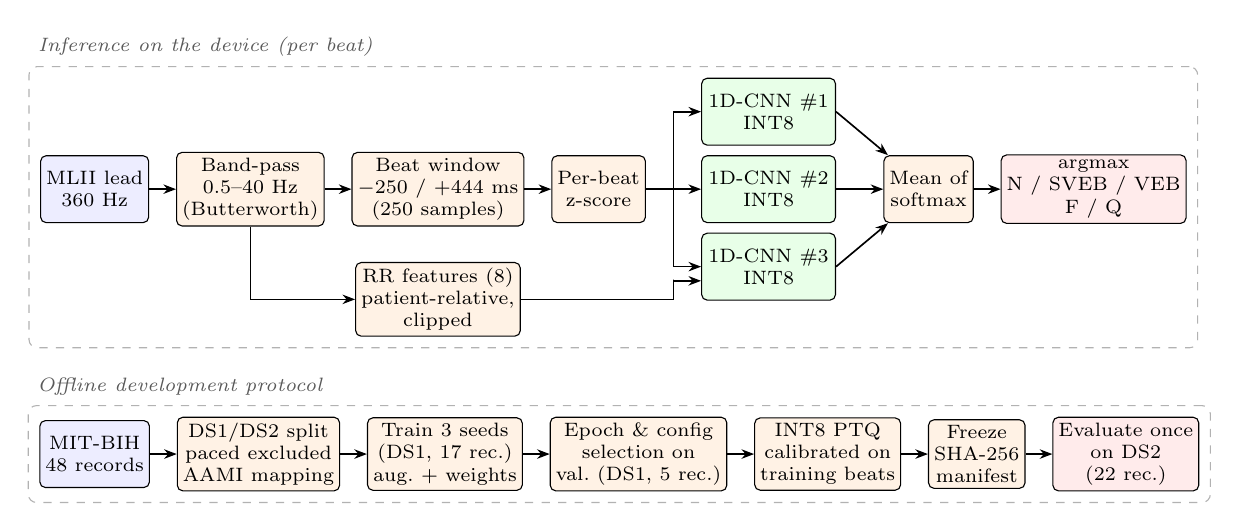
\begin{tikzpicture}[node distance=3.5mm and 3.4mm]
% inference lane
\node[sDATA] (ecg) {MLII lead\\360 Hz};
\node[sPROC, right=of ecg] (bp) {Band-pass\\0.5--40 Hz\\(Butterworth)};
\node[sPROC, right=of bp] (seg) {Beat window\\$-$250 / +444 ms\\(250 samples)};
\node[sPROC, right=of seg] (z) {Per-beat\\z-score};
\node[sPROC, below=of seg, yshift=-1mm] (rr) {RR features (8)\\patient-relative,\\clipped};
\node[sNET, right=7mm of z, minimum width=17mm] (m2) {1D-CNN \#2\\INT8};
\node[sNET, above=1.2mm of m2, minimum width=17mm] (m1) {1D-CNN \#1\\INT8};
\node[sNET, below=1.2mm of m2, minimum width=17mm] (m3) {1D-CNN \#3\\INT8};
\node[sPROC, right=6mm of m2] (avg) {Mean of\\softmax};
\node[sOUT, right=of avg] (cls) {argmax\\N / SVEB / VEB\\F / Q};
\draw[arr] (ecg) -- (bp);
\draw[arr] (bp) -- (seg);
\draw[arr] (seg) -- (z);
\draw[arr] (bp.south) |- (rr.west);
\coordinate (fan) at ($(z.east)!0.5!(m2.west)$);
\draw[arr] (z.east) -- (fan) |- (m1.west);
\draw[arr] (fan) -- (m2.west);
\draw[arr] (fan) |- (m3.west);
\draw[arr] (rr.east) -| ($(fan)+(0,-11.5mm)$) |- ($(m3.west)+(0,-1.8mm)$);
\draw[arr] (m1.east) -- (avg);
\draw[arr] (m2.east) -- (avg);
\draw[arr] (m3.east) -- (avg);
\draw[arr] (avg) -- (cls);
\begin{scope}[on background layer]
\node[lane, fit=(ecg)(cls)(m1)(m3)(rr)] (lane1) {};
\end{scope}
\node[lanelabel] at (lane1.north west) {Inference on the device (per beat)};
% development lane
\node[sDATA, below=25mm of ecg] (db) {MIT-BIH\\48 records};
\node[sPROC, right=of db] (split) {DS1/DS2 split\\paced excluded\\AAMI mapping};
\node[sPROC, right=of split] (train) {Train 3 seeds\\(DS1, 17 rec.)\\aug.\ + weights};
\node[sPROC, right=of train] (sel) {Epoch \& config\\selection on\\val.\ (DS1, 5 rec.)};
\node[sPROC, right=of sel] (ptq) {INT8 PTQ\\calibrated on\\training beats};
\node[sPROC, right=of ptq] (frz) {Freeze\\SHA-256\\manifest};
\node[sOUT, right=of frz] (ds2) {Evaluate once\\on DS2\\(22 rec.)};
\foreach \a/\b in {db/split, split/train, train/sel, sel/ptq, ptq/frz, frz/ds2} \draw[arr] (\a) -- (\b);
\begin{scope}[on background layer]
\node[lane, fit=(db)(ds2)] (lane2) {};
\end{scope}
\node[lanelabel] at (lane2.north west) {Offline development protocol};
\end{tikzpicture}
\caption{System overview. Top: per-beat inference with a three-member INT8 ensemble; the beat and its RR features feed every member. Bottom: development protocol; DS2 is used only after the model is frozen.}
\label{fig:system}
\end{figure*}

\subsection{Dataset and Inter-Patient Protocol}
We use the MIT-BIH Arrhythmia Database~\cite{moody2001impact,goldberger2000physiobank}, obtained from PhysioNet and verified against its published SHA-256 checksums (all 144 record, header and annotation files matched). The paced records 102, 104, 107 and 217 are excluded. Annotation symbols are mapped to AAMI classes as N\,=\,\{N, L, R, e, j\}, SVEB\,=\,\{A, a, J, S\}, VEB\,=\,\{V, E\}, F\,=\,\{F\} and Q\,=\,\{/, f, Q\}~\cite{aami2012ec57}. Records follow the DS1/DS2 split of~\cite{dechazal2004automatic}. Five DS1 records, chosen so that SVEB, VEB and F all occur, form a patient-wise validation set used for every training and design decision. Record 208, which holds most DS1 F beats, stays in training. Table~\ref{tab:data} lists the splits; Fig.~\ref{fig:classdist} shows the class imbalance.

Our per-class beat counts match the reference counts of~\cite{dechazal2004automatic} to within 0.1\%. The small difference comes from discarding the first and last beat of each record, whose RR intervals are undefined, and beats whose window would cross the record boundary.

\begin{table}[t]
\caption{Data Splits and Beat Counts per AAMI Class}
\label{tab:data}
\centering
\footnotesize
\setlength{\tabcolsep}{2.6pt}
\begin{tabular}{@{}lrrrrrrr@{}}
\toprule
Split & Rec. & Beats & N & SVEB & VEB & F & Q \\
\midrule
Train (DS1) & 17 & 40,066 & 36,527 & 552 & 2,581 & 398 & 8 \\
Validation (DS1) & 5 & 10,911 & 9,297 & 391 & 1,207 & 16 & 0 \\
Test (DS2) & 22 & 49,668 & 44,218 & 1,836 & 3,219 & 388 & 7 \\
\bottomrule
\end{tabular}
\\[2pt]\parbox{\columnwidth}{\scriptsize Validation records: 106, 118, 201, 220, 223. Training: 101, 108, 109, 112, 114, 115, 116, 119, 122, 124, 203, 205, 207, 208, 209, 215, 230. Test (DS2): 100, 103, 105, 111, 113, 117, 121, 123, 200, 202, 210, 212, 213, 214, 219, 221, 222, 228, 231, 232, 233, 234.}
\end{table}

\begin{figure}[t]
\centering
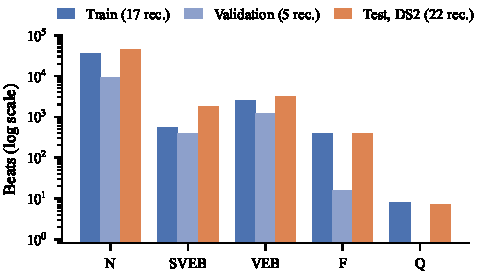
\includegraphics[width=\columnwidth]{class_distribution}
\caption{Beats per AAMI class and split (log scale). Class N is about 89\% of all beats; Q is almost absent.}
\label{fig:classdist}
\end{figure}

\subsection{Preprocessing and Beat Segmentation}
The MLII lead is selected by name (it is the second channel in record 114). It is filtered by a fourth-order zero-phase Butterworth band-pass filter (0.5--40~Hz), which removes baseline wander from respiration and high-frequency noise. Around each annotated R-peak $r$ we cut the window $[r-90, r+160)$ samples, about 250~ms before and 444~ms after the peak, and normalize each beat $\mathbf{x}$ independently:
\begin{equation}
\tilde{\mathbf{x}} = (\mathbf{x}-\mu_{\mathbf{x}})/(\sigma_{\mathbf{x}}+\epsilon),
\end{equation}
so that the network focuses on shape rather than on the patient-dependent amplitude. Fig.~\ref{fig:beats} shows the mean training beat of each class. Like most inter-patient studies, we use the reference R-peak annotations; a deployed system needs an R-peak detector.

\begin{figure*}[t]
\centering
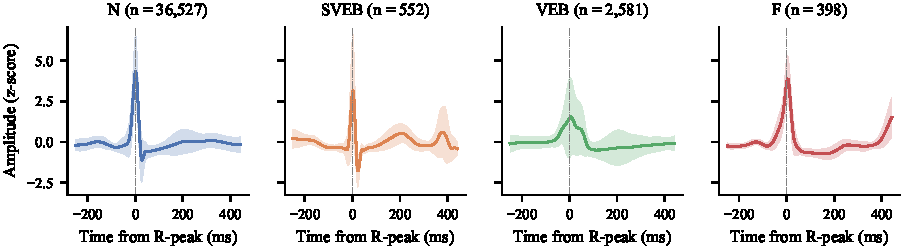
\includegraphics[width=\textwidth]{beat_morphology}
\caption{Mean $\pm$ one standard deviation of the normalized training beats per class. VEB beats are wide and without a preceding P-wave; SVEB beats look almost normal, so their detection relies mainly on timing.}
\label{fig:beats}
\end{figure*}

\subsection{RR-Interval Features}
SVEB beats differ little from normal beats in shape (Fig.~\ref{fig:beats}) but arrive early. With beat times $t_i$ we compute the previous and next intervals $RR^{\mathrm{pre}}_i=t_i-t_{i-1}$ and $RR^{\mathrm{post}}_i=t_{i+1}-t_i$. We also compute the local mean $\overline{RR}^{\mathrm{loc}}_i$ of the previous 10 intervals and the long-term mean $\overline{RR}^{\mathrm{long}}_i$ over the preceding 5~min. Both averages use past beats only. The eight inputs are the four intervals and the ratios
\begin{equation}
\frac{RR^{\mathrm{pre}}_i}{\overline{RR}^{\mathrm{long}}_i},\;
\frac{RR^{\mathrm{post}}_i}{\overline{RR}^{\mathrm{long}}_i},\;
\frac{\overline{RR}^{\mathrm{loc}}_i}{\overline{RR}^{\mathrm{long}}_i},\;
\frac{RR^{\mathrm{pre}}_i}{RR^{\mathrm{post}}_i}.
\end{equation}
The ratios compare each beat with \emph{the patient's own} rhythm, so a ratio of 0.7 means a beat 30\% earlier than usual for this patient at any baseline heart rate. Fig.~\ref{fig:rr} shows the resulting separation. Only $RR^{\mathrm{post}}$ needs the next beat, which delays each decision by one beat (under 1~s); Section~\ref{sec:ablation} evaluates a variant without it.

Gaps in the beat annotations (unreadable signal stretches) produce apparent intervals of up to 100~s. These distorted the normalization statistics and, after quantization, stretched the shared INT8 range of the RR input to 0--11.24 in steps of 0.044. That step is too coarse to separate a prematurity ratio of 0.75 from 0.8. We therefore clip intervals to 0.2--2.0~s (30--300~bpm) and ratios to 0--3. This shrinks the INT8 step to 0.012 and is applied identically in training, testing and on the device. The RR inputs are standardized by a normalization layer whose training-set mean and variance are stored inside the model.

\begin{figure}[t]
\centering
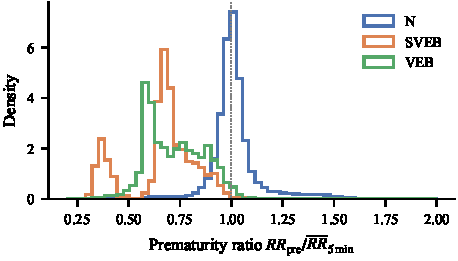
\includegraphics[width=\columnwidth]{rr_prematurity}
\caption{Distribution of the prematurity ratio on the training set. SVEB and VEB beats arrive early relative to the patient's 5-min mean.}
\label{fig:rr}
\end{figure}

\subsection{Network Architecture}
Each ensemble member (Fig.~\ref{fig:arch}) has a morphology branch and a timing branch. The morphology branch has three blocks of Conv1D (8, 16 and 32 filters; kernels 7, 5 and 5; no bias), batch normalization, ReLU and max-pooling by 2, followed by global average pooling. The timing branch normalizes the RR inputs. The two branches are concatenated (40 features) and pass through a 32-unit ReLU layer, dropout of 0.2 and a five-way softmax. The network has 4,974 parameters (Table~\ref{tab:arch}).

\begin{figure}[t]
\centering
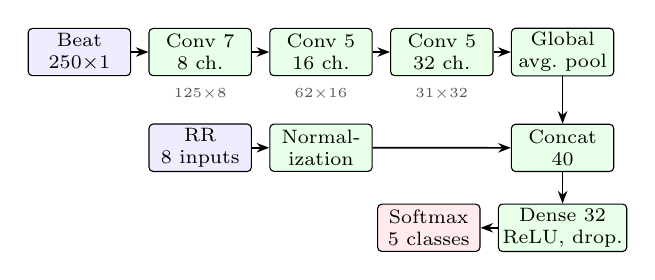
\begin{tikzpicture}[node distance=2.2mm, every node/.style={font=\scriptsize}]
\tikzset{L/.style={draw, rounded corners=1.5pt, fill=green!9, minimum width=13mm, minimum height=6mm, align=center, inner sep=1.5pt},
         I/.style={L, fill=blue!7}, O/.style={L, fill=red!8}}
\node[I] (in) {Beat\\250$\times$1};
\node[L, right=of in] (c1) {Conv 7\\8 ch.};
\node[L, right=of c1] (c2) {Conv 5\\16 ch.};
\node[L, right=of c2] (c3) {Conv 5\\32 ch.};
\node[L, right=of c3] (gap) {Global\\avg.\ pool};
\node[I, below=6mm of c1] (rr) {RR\\8 inputs};
\node[L, right=of rr] (nm) {Normal-\\ization};
\node[L, below=6mm of gap] (cat) {Concat\\40};
\node[L, below=4mm of cat] (fc) {Dense 32\\ReLU, drop.};
\node[O, left=of fc] (sm) {Softmax\\5 classes};
\draw[arr] (in) -- (c1); \draw[arr] (c1) -- (c2); \draw[arr] (c2) -- (c3); \draw[arr] (c3) -- (gap);
\draw[arr] (gap) -- (cat); \draw[arr] (rr) -- (nm); \draw[arr] (nm) -- (cat); \draw[arr] (cat) -- (fc); \draw[arr] (fc) -- (sm);
\node[below=0.3mm of c1, font=\tiny, text=gray!70!black] {125$\times$8};
\node[below=0.3mm of c2, font=\tiny, text=gray!70!black] {62$\times$16};
\node[below=0.3mm of c3, font=\tiny, text=gray!70!black] {31$\times$32};
\end{tikzpicture}
\caption{One ensemble member. Each conv block is Conv1D, batch normalization, ReLU and max-pooling by 2 (output sizes in grey).}
\label{fig:arch}
\end{figure}

\begin{table}[t]
\caption{Layers of One Ensemble Member}
\label{tab:arch}
\centering
\footnotesize
\begin{tabular}{@{}lrr@{}}
\toprule
Layer & Output & Params \\
\midrule
Conv1D(8, $k$=7), BN, ReLU, pool & 125$\times$8 & 56 + 32 \\
Conv1D(16, $k$=5), BN, ReLU, pool & 62$\times$16 & 640 + 64 \\
Conv1D(32, $k$=5), BN, ReLU, pool & 31$\times$32 & 2,560 + 128 \\
Global average pooling & 32 & 0 \\
RR normalization (stored stats) & 8 & 17 \\
Concat, Dense(32), ReLU, dropout & 32 & 1,312 \\
Dense(5), softmax & 5 & 165 \\
\midrule
Total (trainable) & & 4,974 (4,845) \\
\bottomrule
\end{tabular}
\end{table}

\subsection{Training}
Class imbalance is handled with per-sample loss weights
\begin{equation}
w_c=\min\!\Big(\big(N/(K\,n_c)\big)^{p},\,w_{\max}\Big),
\end{equation}
where $n_c$ is the number of training beats of class $c$, $K=5$, $w_{\max}=25$, and the exponent $p$ is chosen on validation. The weighted cross-entropy is minimized with Adam~\cite{kingma2015adam} (initial learning rate $2\times10^{-3}$, batch size 256) and a cosine learning-rate decay~\cite{loshchilov2017sgdr} over at most 60 epochs. Training-time augmentation applies five transformations: amplitude scaling ($\times$0.8--1.2), Gaussian noise ($\sigma$\,=\,0.05), a random linear baseline drift, a time shift of up to $\pm$5 samples (mimicking R-peak detector jitter), and a joint heart-rate rescaling of the absolute RR intervals ($\times$0.85--1.15), which leaves the ratios unchanged. After every epoch the model is scored on the validation set. The selection score is the macro-F1 over N, SVEB and VEB, because the validation set holds only 16 F beats and no Q beats. The best epoch is kept, with early stopping after 15 epochs without improvement. Every configuration is trained with three seeds, and results are reported as mean $\pm$ standard deviation.

\subsection{Evaluation Metrics}
Following EC57, we report gross (pooled over all test beats) per-class
\begin{equation}
\mathrm{Se}=\tfrac{TP}{TP+FN},\quad +P=\tfrac{TP}{TP+FP},\quad \mathrm{FPR}=\tfrac{FP}{FP+TN},
\end{equation}
together with accuracy and the macro-F1 over N, SVEB, VEB and F. Q has seven test beats, so no Q claim is made.

\subsection{Quantization and Cost Estimation}
For full-integer post-training quantization (PTQ), real values are represented as $r=S(q-Z)$ with 8-bit $q$~\cite{jacob2018quantization}. Weights use per-channel scales; activations and the model inputs and outputs use per-tensor scales calibrated on 2,000 training beats. Batch normalization is folded into the preceding convolution,
\begin{equation}
W'=W\,\tfrac{\gamma}{\sqrt{\sigma^2+\epsilon}},\qquad b'=\beta-\tfrac{\mu\gamma}{\sqrt{\sigma^2+\epsilon}}.
\end{equation}
For quantization-aware training (QAT), the network is rebuilt in exactly the graph TensorFlow Lite executes (folded (1$\times k$) Conv2D layers). Fake quantization is inserted on the convolutions, the ReLUs and the dense layers. Activation ranges are calibrated before fine-tuning, and the fine-tuning epoch is selected on validation. Multiply-accumulates (MACs) are counted from the converted graph as $L_{\mathrm{out}}\,k\,C_{\mathrm{in}}C_{\mathrm{out}}$ per convolution and $d_{\mathrm{in}}d_{\mathrm{out}}$ per dense layer. Peak activation memory is the maximum, over the execution order, of the bytes of all simultaneously live activation tensors. Weights stay in flash, so this is a lower bound on the TensorFlow Lite Micro~\cite{david2021tflm} tensor arena, which adds alignment and bookkeeping.

\subsection{Ensemble and Decision Rule}
Training with different seeds produced large differences in minority-class results, so the final classifier averages the dequantized softmax outputs of the $M=3$ INT8 members~\cite{lakshminarayanan2017ensembles},
\begin{equation}
\hat{y}=\arg\max_c \tfrac{1}{M}\textstyle\sum_{m=1}^{M} p_m(c\mid\mathbf{x}).
\end{equation}
On a microcontroller the members run one after another in the same tensor arena, so peak RAM stays that of one member while weights and MACs add up. We also tested a validation-tuned SVEB threshold (SVEB only if $\bar{p}(\mathrm{SVEB})\ge t$) and two ablations (Section~\ref{sec:ablation}). The selection rule was fixed before the candidates' validation results were seen: the INT8 ensemble with the highest validation F1 over N, SVEB and VEB wins. The chosen model was then frozen with a SHA-256 manifest and evaluated once on DS2 by a script that refuses to run twice.

%=====================================================================
\section{Results}
%=====================================================================
\subsection{Model Selection on Validation}
Table~\ref{tab:sweep} summarizes the validation sweep. Balanced weights ($p=1$) gave the best selection score, and augmentation reduced its seed-to-seed spread from $\pm$2.48 to $\pm$0.10. RR clipping raised SVEB sensitivity from 60.6\% to 65.4\% and the score from 76.10 to 77.03, so the final configuration is $p=1$ with augmentation and clipping. Fig.~\ref{fig:curves} shows its training curves. The best epochs (10, 4 and 5) come early, consistent with fast overfitting to the 17 training patients.

\begin{table}[t]
\caption{Validation Sweep (Mean $\pm$ SD over Three Seeds, \%)}
\label{tab:sweep}
\centering
\footnotesize
\setlength{\tabcolsep}{2.4pt}
\resizebox{\ifdim\width>\columnwidth\columnwidth\else\width\fi}{!}{%
\begin{tabular}{@{}cccccccc@{}}
\toprule
$p$ & Aug. & Clip & F1$_{\mathrm{N,S,V}}$ & SVEB Se & SVEB +P & VEB Se & VEB +P \\
\midrule
0.5 & & & 74.94$\pm$1.26 & 49.7$\pm$14.6 & 40.8 & 85.7 & 89.0 \\
0.5 & \cmark & & 74.71$\pm$1.79 & 54.7$\pm$6.3 & 35.8 & 85.3 & 89.4 \\
0.75 & \cmark & & 75.62$\pm$2.46 & 51.4$\pm$5.0 & 40.1 & 86.4 & 89.8 \\
1.0 & & & 77.06$\pm$2.48 & 52.7$\pm$10.7 & 45.3 & 85.1 & 91.8 \\
1.0 & \cmark & & 76.10$\pm$0.10 & 60.6$\pm$5.5 & 35.0 & 85.6 & 91.3 \\
\textbf{1.0} & \cmark & \cmark & \textbf{77.03$\pm$0.85} & \textbf{65.4$\pm$7.5} & 37.1 & 86.7 & 91.5 \\
\bottomrule
\end{tabular}}
\end{table}

\begin{figure}[t]
\centering
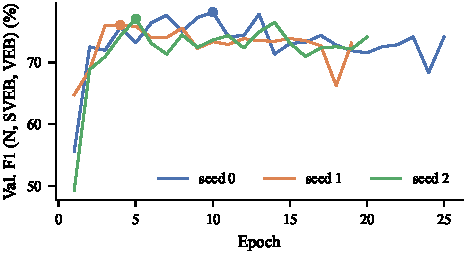
\includegraphics[width=\columnwidth]{training_curves}
\caption{Validation selection score per epoch for the three seeds of the final configuration; dots mark the kept epochs.}
\label{fig:curves}
\end{figure}

\subsection{Inter-Patient Test Results}
Table~\ref{tab:final} reports the frozen INT8 ensemble on DS2 and Fig.~\ref{fig:cm} its confusion matrix. VEB is detected reliably (Se 92.89\%, +P 92.71\%, FPR 0.51\%). SVEB sensitivity is 74.46\%, but only one SVEB call in three is correct. F beats are not recognized, and the reasons are discussed in Section~\ref{sec:discussion}.

\begin{table}[t]
\caption{Frozen INT8 Ensemble on DS2 (Inter-Patient, \%)}
\label{tab:final}
\centering
\footnotesize
\begin{tabular}{@{}lrrrr@{}}
\toprule
Class & Beats & Se & +P & FPR \\
\midrule
N & 44,218 & 88.21 & 97.77 & 16.33 \\
SVEB & 1,836 & 74.46 & 33.43 & 5.69 \\
VEB & 3,219 & 92.89 & 92.71 & 0.51 \\
F & 388 & 0.00 & 0.00 & 4.98 \\
Q & 7 & 0.00 & 0.00 & 0.02 \\
\bottomrule
\end{tabular}
\\[2pt]\parbox{\columnwidth}{\centering\footnotesize Accuracy 87.30, macro-F1 (N, SVEB, VEB, F) 57.92}
\end{table}

\begin{figure}[t]
\centering
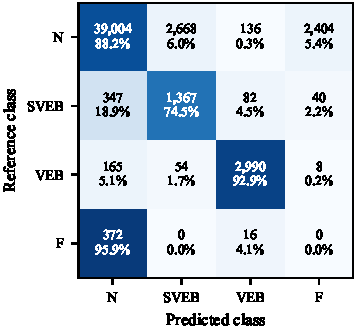
\includegraphics[width=0.8\columnwidth]{confusion_ds2}
\caption{DS2 confusion matrix of the frozen INT8 ensemble (counts and row percentages; Q omitted, 7 beats).}
\label{fig:cm}
\end{figure}

Table~\ref{tab:ensemble} compares single members with the ensemble. The ensemble beats the mean single model on every listed metric, in both FP32 and INT8. Most importantly, it replaces an SVEB sensitivity that varies by $\pm$14 points across seeds with a single deterministic result.

\begin{table*}[t]
\caption{Single Members (Mean $\pm$ SD, $n=3$) Versus the Ensemble on DS2 (\%)}
\label{tab:ensemble}
\centering
\footnotesize
\begin{tabular}{@{}lcccccccc@{}}
\toprule
Model & Accuracy & Macro-F1 & N Se & N FPR & SVEB Se & SVEB +P & VEB Se & VEB +P \\
\midrule
FP32, single & 85.72$\pm$2.52 & 56.72$\pm$0.45 & 86.46$\pm$2.78 & 15.74$\pm$3.03 & 76.33$\pm$12.96 & 31.46$\pm$1.76 & 91.44$\pm$4.05 & 90.88$\pm$2.84 \\
FP32, ensemble & 87.39 & 58.25 & 88.04 & 14.07 & 80.99 & 33.65 & 92.85 & 92.48 \\
INT8, single & 85.70$\pm$2.73 & 56.31$\pm$0.63 & 86.66$\pm$3.02 & 17.73$\pm$2.88 & 71.11$\pm$13.98 & 30.93$\pm$1.26 & 91.27$\pm$3.96 & 90.73$\pm$3.08 \\
\textbf{INT8, ensemble (final)} & \textbf{87.30} & \textbf{57.92} & \textbf{88.21} & \textbf{16.33} & \textbf{74.46} & \textbf{33.43} & \textbf{92.89} & \textbf{92.71} \\
\bottomrule
\end{tabular}
\end{table*}

\subsection{Quantization and Embedded Feasibility}
Table~\ref{tab:quant} gives the cost of one member (seed 0) in FP32, PTQ and QAT, and of the final ensemble. INT8 shrinks the weights 3.7$\times$, from 18.8~KB to 5.0~KB, and peak activation memory 4$\times$, from 15.7~KB to 3.9~KB (Fig.~\ref{fig:mem}). The accuracy cost is 0.5--0.6 points; Fig.~\ref{fig:quant} breaks it down by class. QAT matched FP32 on validation already before fine-tuning (validation score 78.0 vs.\ 78.1), so fine-tuning selected epoch 0 and QAT brought no accuracy gain. Its smaller file and activation footprint come from the leaner exported graph, which has fewer reshape operators. The only noticeable quantization cost is SVEB sensitivity (78.4\% to 72.1\% for one member, 81.0\% to 74.5\% for the ensemble); VEB and N are essentially unchanged.

\begin{table}[t]
\caption{Model Cost and DS2 Accuracy Before and After Quantization}
\label{tab:quant}
\centering
\footnotesize
\setlength{\tabcolsep}{2.5pt}
\resizebox{\ifdim\width>\columnwidth\columnwidth\else\width\fi}{!}{%
\begin{tabular}{@{}lrrrrrr@{}}
\toprule
Model & File & Weights & MACs & Peak act. & Acc. & SVEB \\
 & (KB) & (KB) & (k) & (KB) & (\%) & Se (\%) \\
\midrule
FP32 (1 member) & 28.9 & 18.8 & 254 & 15.7 & 83.46 & 78.38 \\
INT8 PTQ (1 member) & 18.6 & 5.0 & 254 & 3.9 & 82.83 & 72.06 \\
INT8 QAT (1 member) & 13.8 & 5.0 & 254 & 2.9 & 82.97 & 72.28 \\
\textbf{INT8 PTQ ensemble} & \textbf{55.9} & \textbf{15.1} & \textbf{762} & \textbf{3.9} & \textbf{87.30} & \textbf{74.46} \\
\bottomrule
\end{tabular}}
\end{table}

\begin{figure}[t]
\centering
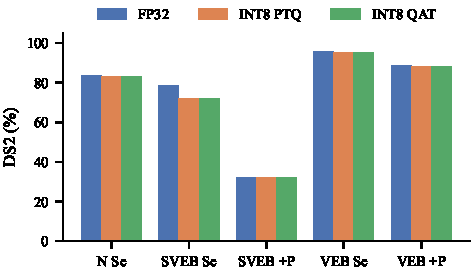
\includegraphics[width=\columnwidth]{quantization}
\caption{DS2 per-class metrics of one member before and after INT8 quantization.}
\label{fig:quant}
\end{figure}

\begin{figure}[t]
\centering
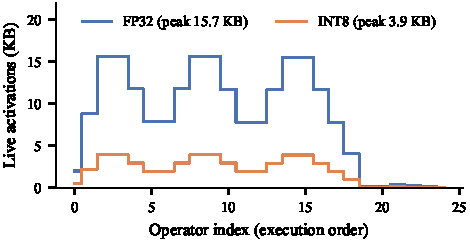
\includegraphics[width=\columnwidth]{memory_timeline}
\caption{Live activation memory per operator in execution order for one member. Weights are excluded (they reside in flash).}
\label{fig:mem}
\end{figure}

Against the ESP32-WROOM-32E~\cite{espressif2023esp32}, the ensemble's activations occupy about 0.8\% of the 520~KB SRAM and its model files about 1.4\% of the smallest (4~MB) flash. At 762k MACs per beat and an assumed 10 clock cycles per MAC (an assumption to be verified on hardware), inference would take about 32~ms per beat at 240~MHz. That is about 4\% of the interval between beats at 75~bpm. For comparison, Kim et al.~\cite{kim2024ultraedge} report 118~kB of RAM for a 25~kB model on a Cortex-M4.

\subsection{Error Analysis: SVEB False Alarms}
Of the 2,668 normal beats called SVEB, 86.5\% come from just five of the 22 test patients (Fig.~\ref{fig:fa}). We read the rhythm annotations of these records: four contain atrial fibrillation or flutter, which covers 37--97\% of their beats, and the fifth (231) has 2:1 AV block. In AF the heart rhythm is irregular throughout, so normal beats often arrive early and match the RR pattern the model associates with SVEB. These errors are confident: the mean SVEB probability of the false alarms is 0.78. A validation-tuned decision threshold therefore cannot remove them. The best threshold ($t=0.51$) improved the validation score by only 0.15 points (Fig.~\ref{fig:thr}), and on DS2 it lowered SVEB sensitivity from 74.46\% to 67.70\% without improving +P (33.05\%). We kept plain argmax.

\begin{figure}[t]
\centering
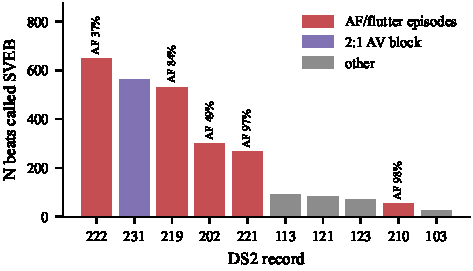
\includegraphics[width=\columnwidth]{false_alarms_by_record}
\caption{Normal beats misclassified as SVEB, by DS2 record (ten largest). The share of beats inside AF/flutter episodes is taken from the MIT-BIH rhythm annotations.}
\label{fig:fa}
\end{figure}

\begin{figure}[t]
\centering
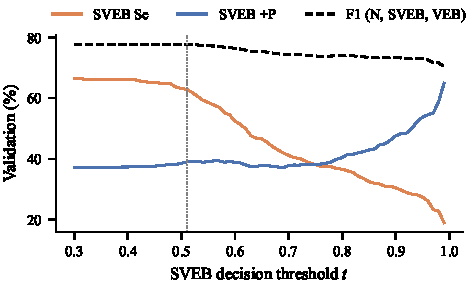
\includegraphics[width=\columnwidth]{threshold_sweep}
\caption{Validation sweep of the SVEB decision threshold. The false alarms are confident, so raising $t$ removes true SVEB detections before it removes false alarms.}
\label{fig:thr}
\end{figure}

\subsection{Ablations}
\label{sec:ablation}
To separate isolated premature beats from irregular rhythms, we added two \emph{rhythm-irregularity} inputs: the coefficient of variation and the mean absolute successive difference of the ten RR intervals \emph{preceding} the current one, both relative to their mean. Leaving out the current interval means a single premature beat does not count as irregularity. On DS1 the feature separates AF beats clearly from sinus-rhythm N and SVEB beats (Fig.~\ref{fig:irreg}). We combined it with global max pooling (``+Irreg.''). A second variant (``Causal'') also drops every input that depends on the next beat, which makes decisions immediate. Both were trained and ensembled with the same protocol. The pre-declared validation rule selected the original model (Table~\ref{tab:ablation}).

On DS2, however, +Irreg.\ is better on every SVEB metric. False alarms fall from 2,668 to 1,916, +P rises from 33.43\% to 42.31\%, sensitivity rises to 77.72\%, and macro-F1 increases by 2.8 points. Our validation set contains no AF patient, so it could not reward a feature whose benefit lies in AF records. Choosing +Irreg.\ now would mean selecting on the test set; it is therefore reported as an ablation, not as our result. The causal variant reaches similar SVEB scores, but it labels 7,242 normal beats as F, so normal-beat sensitivity falls to 78.02\%. Removing the one-beat delay is not worth this cost.

\begin{figure}[t]
\centering
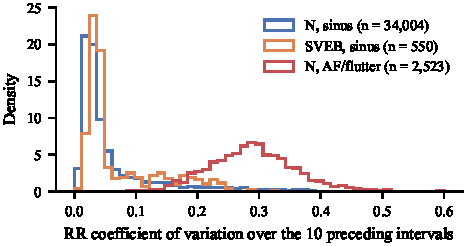
\includegraphics[width=\columnwidth]{rr_irregularity}
\caption{Rhythm irregularity (training set) inside and outside AF/flutter episodes, from the MIT-BIH rhythm annotations.}
\label{fig:irreg}
\end{figure}

\begin{table}[t]
\caption{Ablations (INT8 Ensembles; Validation Selects, DS2 Reports, \%)}
\label{tab:ablation}
\centering
\footnotesize
\setlength{\tabcolsep}{2.2pt}
\resizebox{\ifdim\width>\columnwidth\columnwidth\else\width\fi}{!}{%
\begin{tabular}{@{}lccccccr@{}}
\toprule
 & Val. & \multicolumn{5}{c}{DS2} & Wts. \\
\cmidrule(lr){2-2}\cmidrule(lr){3-7}
Model & F1$_{\mathrm{N,S,V}}$ & mF1 & S Se & S +P & V +P & N Se & (KB) \\
\midrule
\textbf{Frozen (selected)} & \textbf{77.60} & 57.92 & 74.46 & 33.43 & 92.71 & 88.21 & 15.1 \\
+Irreg.\ +max-pool & 74.76 & 60.75 & 77.72 & 42.31 & 91.83 & 89.64 & 18.3 \\
Causal +Irreg. & 76.00 & 57.93 & 78.10 & 39.56 & 86.64 & 78.02 & 18.0 \\
\bottomrule
\end{tabular}}
\end{table}

\subsection{Comparison with Published Work}
Table~\ref{tab:compare} places our result next to studies discussed above, separating results on the canonical DS1/DS2 split from other partitions. On SVEB, our sensitivity matches de Chazal et al.~\cite{dechazal2004automatic} (75.9\%), but our positive predictivity is lower (33.4\% vs.\ 38.5\%). On VEB, our model is clearly stronger (92.9/92.7\% vs.\ 77.7/81.9\%). Among studies with embedded evidence, ours is the only one that combines the canonical inter-patient split with a microcontroller-class memory footprint.

\begin{table}[t]
\caption{Comparison with Published Work}
\label{tab:compare}
\centering
\footnotesize
\setlength{\tabcolsep}{2.2pt}
\resizebox{\ifdim\width>\columnwidth\columnwidth\else\width\fi}{!}{%
\begin{tabular}{@{}llccl@{}}
\toprule
Ref. & Split & SVEB Se/+P & VEB Se/+P & Footprint \\
\midrule
\cite{dechazal2004automatic} & DS1/DS2 & 75.9 / 38.5 & 77.7 / 81.9 & -- (linear disc.) \\
\cite{sahatchinda2025lightweight} & Inter-pat. & \multicolumn{2}{c}{Acc.\ 98.42, Se 87.60$^{b}$} & not reported \\
\cite{kim2024ultraedge} & Subject-wise & \multicolumn{2}{c}{Acc.\ 87.1$^{b}$} & 25~kB, 118~kB RAM \\
\cite{farag2023tiny} & Inter-pat. & \multicolumn{2}{c}{--} & 15~kB, 12--24~MB RAM \\
\cite{busia2025tiny} & Intra-pat. & \multicolumn{2}{c}{Acc.\ 98.97$^{b}$} & 6.6k params, GAP9 \\
\midrule
\textbf{Ours} & \textbf{DS1/DS2} & \textbf{74.5 / 33.4} & \textbf{92.9 / 92.7} & \textbf{15.1~KB, 3.9~KB act.} \\
\bottomrule
\multicolumn{5}{@{}l@{}}{\scriptsize $^{b}$Overall figures as summarized in~\cite{silva2026review}; per-class values not comparable.}
\end{tabular}}
\end{table}

%=====================================================================
\section{Discussion}
\label{sec:discussion}
%=====================================================================
\textbf{Gaps addressed.} The model is AAMI-compliant, evaluated on the canonical inter-patient split and costed against a microcontroller budget (G1--G3). Size, MACs and peak activation memory are reported in one consistent format (G4), and per-class metrics are reported for every class, including the failures (G5). Its 87.3\% accuracy is lower than the 95--99\% common in the literature, but it is measured on unseen patients. Most higher figures come from intra-patient splits.

\textbf{Fusion beats.} No configuration learned F in a way that transfers. Almost all F training beats (372 of 398) come from a single patient (record 208), while most test F beats come from another (record 213). The model learns that patient rather than fusion morphology. This failure is common under the inter-patient protocol and is the clearest example of gap G5.

\textbf{Use of the test set.} DS2 was evaluated seven times during development. These were the first baseline, the tuned configuration before RR clipping, the quantization comparison, the retrained configuration, the ensemble, the threshold check and the frozen model with its ablations. One design change followed a DS2 observation. The quantization comparison exposed an SVEB drop, which we traced to the RR input range and fixed by clipping. Clipping removes a physiological artefact (annotation gaps), and it also improved validation sensitivity by 4.8 points, but the DS2 results are not a strictly untouched estimate. Every other choice was made on validation, and the frozen model was evaluated exactly once.

\textbf{Other limitations.} Records 201 (in our validation set) and 202 (in DS2) come from the same patient, an accepted exception of the canonical split. The validation set has no AF patient, which is why the irregularity feature could not be selected. We use reference R-peak annotations rather than a detector. Embedded costs are estimated from the converted graphs, not yet measured on the ESP32.

%=====================================================================
\section{Conclusion and Future Work}
%=====================================================================
We presented a three-member INT8 1D-CNN ensemble for five-class AAMI heartbeat classification that meets all three E3C criteria. On unseen patients it detects 92.9\% of ventricular and 74.5\% of supraventricular ectopic beats. It needs 15.1~KB of weights and about 4~KB of working memory, and quantization costs almost no accuracy. The main remaining weakness, SVEB false alarms, is concentrated in atrial-fibrillation patients. A rhythm-irregularity feature addresses it effectively, but its benefit is visible only with AF patients in the validation data. Future work will (i) rebuild the validation protocol with AF records, or use cross-validation over DS1 patients, before re-selecting; (ii) deploy the frozen model with TensorFlow Lite Micro on an ESP32-WROOM-32E and measure latency, arena size and energy; (iii) add an on-device R-peak detector; and (iv) study F-class generalization, for example with data from additional databases.

\bibliographystyle{IEEEtran}
\bibliography{refs}

\end{document}
